\newpage
\singlespacing

\textbf{Lampiran 1. Model FE}

\begin{table}[h]
\centering
    \begin{tabular}[t]{p{7cm}cccc}
    \toprule
    ln Produk Domestik Regional Bruto & $\hat{\beta}$ & $se(\hat{\beta})$ & Sig & 95\%CI \\
    \midrule
    ln Pembentukkan Modal Tetap Bruto & 0.384  & 0.077  & ***  & 0.233 - 0.536 \\
    ln Angka Partisipasi Kasar Sekolah Menengah & 0.103  & 0.043  & *    & 0.018 - 0.189 \\
    ln Tingkat Kesempatan Kerja & 1.254  & 0.468  & **   & 0.329 - 2.179 \\
    ln Tingkat Penetrasi Internet & 0.149  & 0.023  & ***  & 0.104 - 0.194 \\
    \midrule
        \multicolumn{4}{l}{Heteroscedasticity and Autocorrelation Consistent standard errors}\\
    \midrule
        \multicolumn{4}{l}{Total Sum of Square = 2.0667} \\
        \multicolumn{4}{l}{Residual Sum of Square = 0.1632} \\
        \multicolumn{4}{l}{$R^{2}= 0.9210$} \\
        \multicolumn{4}{l}{$F(4, 161) = 469.454$} \\
    \midrule
        \multicolumn{4}{l}{Catatan: *** p<0.001, ** p<0.01, * p<0.05, ln : logaritma natural}\\
    \bottomrule
    \end{tabular}
\end{table}


\textbf{Lampiran 2. Hasil Pengujian}

\begin{center}
\begin{tabular}{cccp{5cm}}
\toprule
Uji                 & Statistik             & p-value  & $H_0$ (Hipotesis nol) \\
\midrule
Chow                & $F(160, 33) = 142.81$ & 0.000    & Intersep dan Slope adalah sama \\
Honda               & $z = 21.084$          & 0.000    & Tidak terdapat efek individu    \\
Hausman             & $\chi^2(4) = 153.54$  & 0.000    & Tidak ada korelasi antar efek individu dengan variabel bebas\\
Breusch-Godfrey AR(1) & $\chi^2(1) = 13.277$  & 0.000    & Tidak ada korelasi serial order ke-1    \\
Breusch-GodfreyAR(6) & $\chi^2(6) = 50.041$  & 0.000    & Tidak ada korelasi serial order ke-6    \\
\bottomrule
\end{tabular}
\end{center}

\newpage
\textbf{Lampiran 3. Heteroskedastisitas galat}

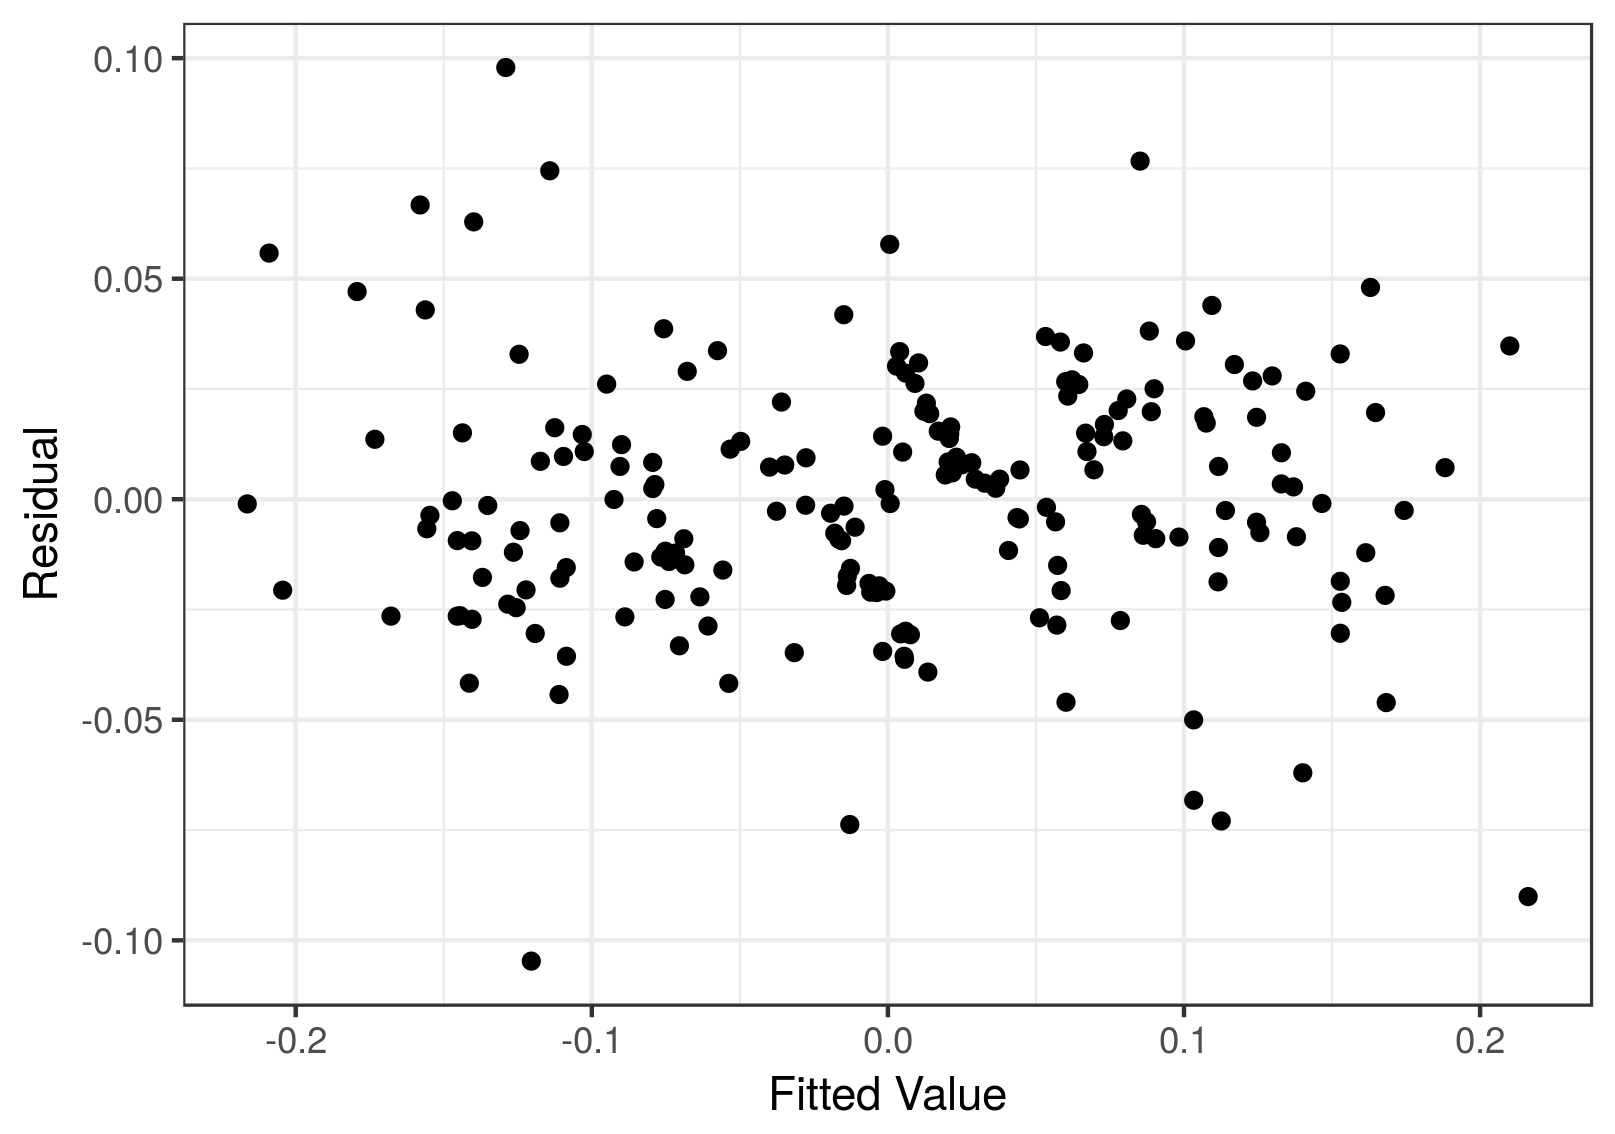
\includegraphics[width = 0.6\textwidth]{img/hetero.png}

\textbf{Lampiran 4. Normal Q-Q plot}

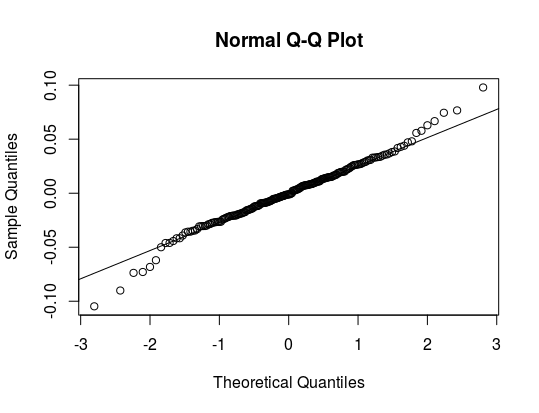
\includegraphics[width = 0.6\textwidth]{img/normal-qqplot.png}

\textbf{Lampiran 5. Density plot residual}

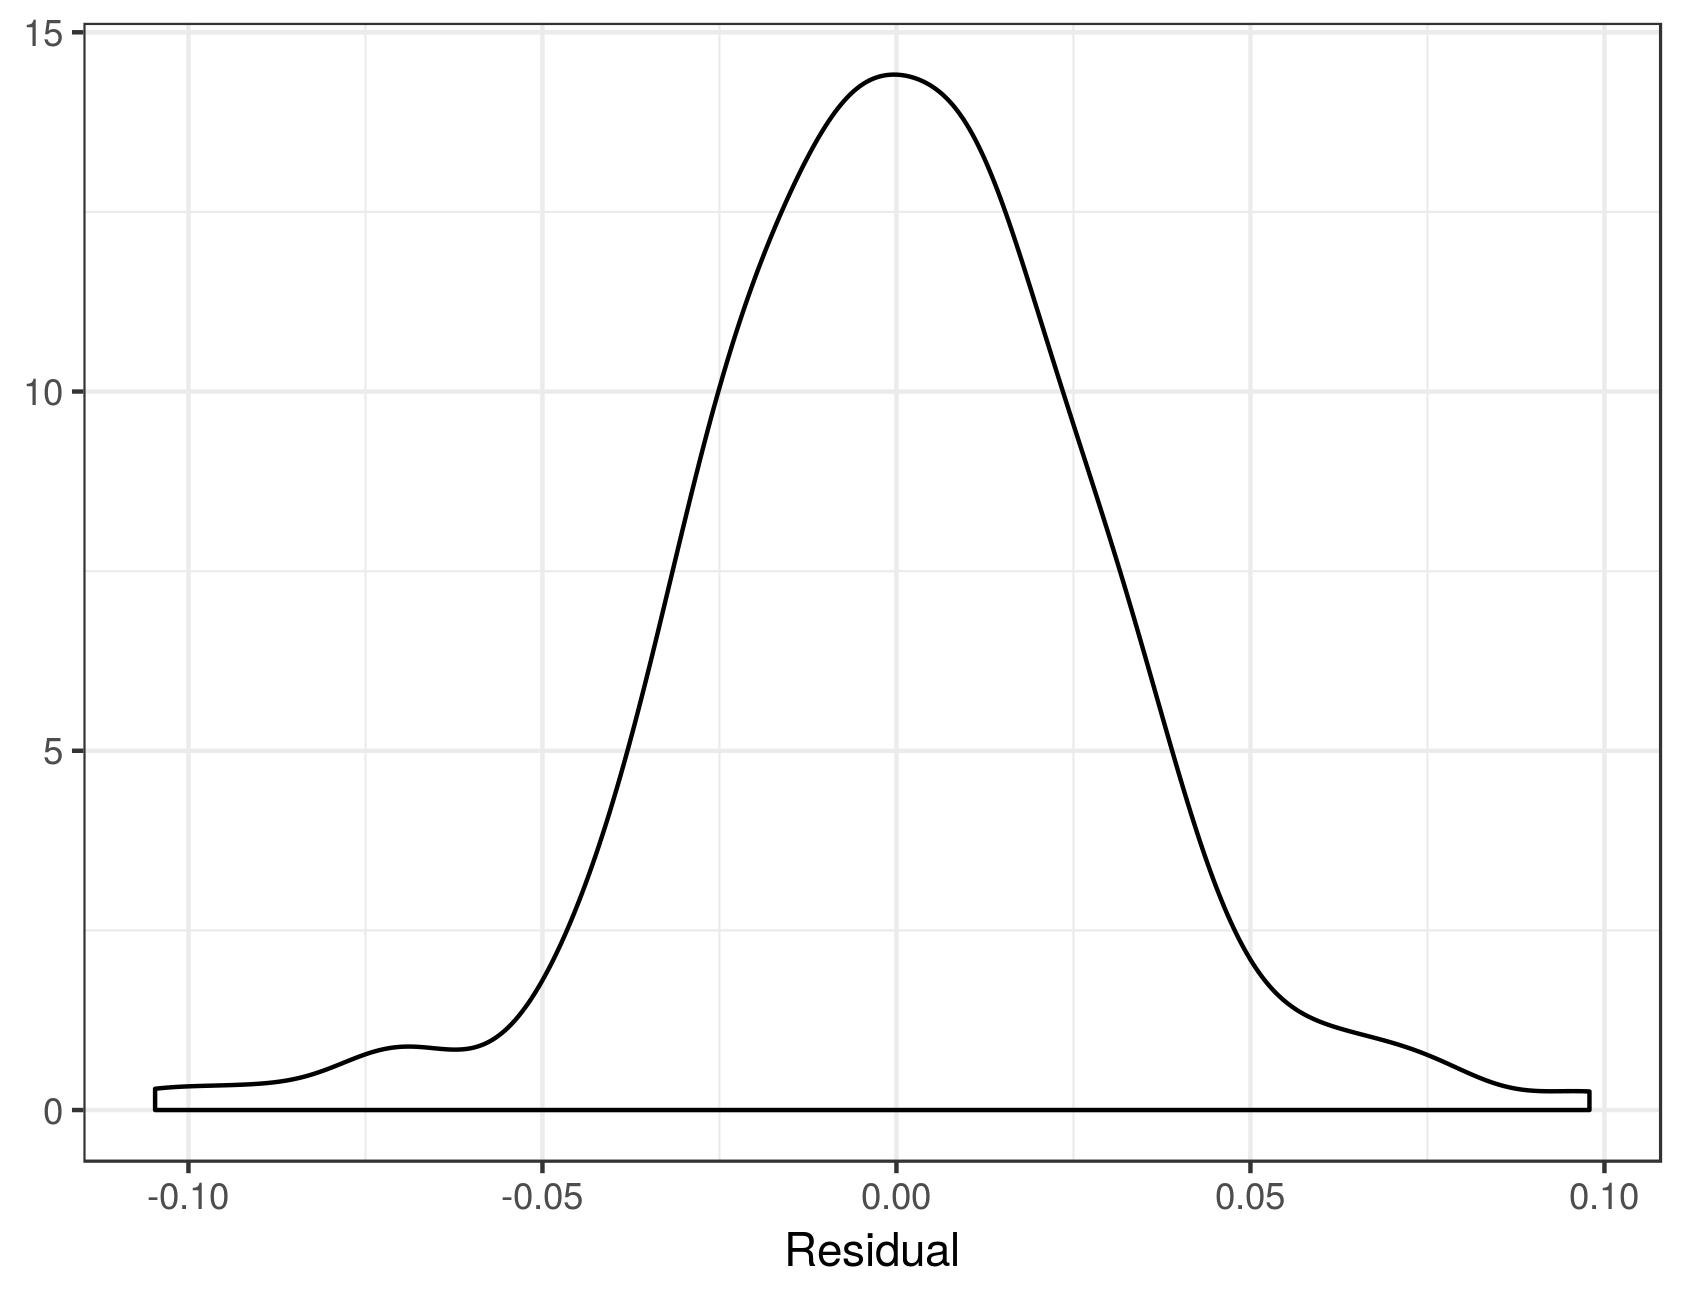
\includegraphics[width = 0.6\textwidth]{img/galat-density.png}

\textbf{Lampiran 6. R script untuk pemodelan}

\begin{verbatim}
library(plm)
library(lmtest)
library(broom)
library(ggplot2)
theme_set(theme_bw())
net <- read.csv("net_clean.csv")

# Jadikan p.dataframe
nep <- pdata.frame(net, index = c("i", "t"), drop.index = F)

# Alpha
alpha <- 0.05

# Spesifikasi Model
f1 <- log(Y) ~ log(K) + log(H) + log(L) + log(I)

# Estimasi model

POLS <- plm(f1, nep, model = "pooling") # Pooled OLS
FE <- plm(f1, nep, model = "within") # Fixed / Within
RE <- plm(f1, nep, model = "random") # Random
VC <- pvcm(f1, nep, model = "within")

# POLS vs FE vs RE -----

# Uji Chow
pooltest(POLS, VC)

# Uji Honda
plmtest(POLS, type = "honda", effect = "individual")

# Uji Hausmann
phtest(FE, RE)

# Heteroskedastisitas Galat
hetero <- qplot(y = resid(FE), x = fitted(FE),
                ylab = "Residual", xlab = "Fitted Value")

# ggsave(plot = hetero, filename = "Lampiran-hetero.png", device = "png")

# Uji Breusch-Godfrey
pbgtest(FE, order = 1)
pbgtest(FE)

# Jarque Bera
normtest::jb.norm.test(resid(FE)); qchisq(1-alpha, 2)

# Density Plot
denseplot <- qplot(resid(FE), geom = "density", xlab = "Residual", ylab = NULL)

# ggsave(plot = denseplot, filename = "Lampiran-galat-density.png", device = "png")

# qqplot
#qqnorm(resid(FE))
#qqline(resid(FE))

# Robust Standard Error HAC
HAC <- vcovHC(FE, method = "arellano")

# Inferensia
library(lmtest)

## Statistik t
coeftest(FE, vcov. = HAC, df = NULL) # Uji Wald
coeftest(FE, vcov. = HAC, df = FE$df.residual) # Uji t

## Selang Kepercayaan
coefci(FE, vcov. = HAC)

## Statistik F
z <- Within(log(nep$Y)) # Transformasi Within
sst <- sum(z^2) # Sum Square Total
df1 <- 4 # df1
ssr <- sum(resid(FE)^2) # Sum Square Residual
df2 <- df.residual(FE) # df residual

F_stat <- ((sst-ssr)/df1)/((ssr)/df2) # Nilai statistik F
pf(F_stat, df1, df2, lower.tail = F) # p-Value

## R-Squared
r.squared(FE) # R-Squared
\end{verbatim}


Source Code untuk makalah ini dapat dilihat pada \href{https://github.com/rexevan/148429}{https://github.com/rexevan/148429}.
